\section{Temporal concepts} \label{tconcepts}
The SAX transformation procedure described in the previous section yields symbolic time-series based on the daily aggregated data from telemetry streams. Having such a symbolic representation, also called in the literature as \textit{symbolic temporal data}, is very adventageous comparing to the real-valued data in terms of easy pattern search, indexing, clustering and low computational and space complexity. 

It is important also to understand a time-intervals temporal data model before introducing concepts and operators. The \textit{time-intervals} are continous groups of discrete time instants and some algorithms and applications operate with them rather than individual points. Time-intervals essentially are sets of two or more continous points and two successive time points define a minimal interval which starts at the earlier point and continues to the latter point inclusevily.

This section built around the technical report by Fabian M\"orchen \cite{citeulike:1748833} which aggregated many of work done in the field of data mining from symbolic temporal data. Two figures taken from this work constitute the Figure \ref{fig:concepts1} and depict hierarchy of time-points (left panel) and time-intervals (right panel) data models, concepts and operators.

The concept of \textit{concurrency} as described by the author explains the closeness of two time-points in time without considering their ordering, - a coincidence of events in time is important. The \textit{synchronicity} is a special case of concurrency where events occur synchonously in time.

The \textit{order}, and \textit{synchronicity} concepts in the Time intervals model are anlogous ones in the Time points model, whether the Time intervals \textit{coincidence} describes an intersection of intervals in time.

The time point operators from the Figure \ref{fig:concepts1}: \textit{before}, \textit{after} and \textit{equals} precizely define the relation of points in time. The \textit{close} operator is a ``fuzzy extension for temporal reasoning'' since it encapsulates other three. Note that some threshold can be used to relax or constrain these operators, for example we can consider points equal to each other even if they are less than $k$ time units apart.


\begin{figure}[tbp]
   \centering
   \includegraphics[height=45mm]{concepts1.eps}
   \caption{The temporal concepts and operators from \cite{citeulike:1748833} for both: time point and time interval data models.}
   \label{fig:concepts1}
\end{figure}